\documentclass{beamer}
\usetheme{Madrid}

\usepackage{amsmath, amssymb, amsthm}
\usepackage{graphicx}
\usepackage{gensymb}
\usepackage[utf8]{inputenc}
\usepackage{hyperref}
\usepackage{tikz}

\title{1.2.23 Matgeo}
\author{AI25BTECH11015 - M Sai Rithik}
\date{}

\begin{document}

\frame{\titlepage}

% Question frame
\begin{frame}
\frametitle{Question}
Represent graphically a displacement of 40 km, $30^{\circ}$ west of south.
\end{frame}

% Coordinate system assumptions
\begin{frame}
\frametitle{Coordinate System}
We choose the coordinate axes such that:
\begin{itemize}
    \item $+x$ axis $\to$ East
    \item $+y$ axis $\to$ North
\end{itemize}
\end{frame}

% Solution steps
\begin{frame}
\frametitle{Solution}
The given displacement has magnitude
\[
|\vec{D}| = 40 \ \text{km}
\]
and direction $30^{\circ}$ west of south.  

\[
\theta = 270^{\circ} - 30^{\circ} = 240^{\circ}.
\]
\end{frame}

\begin{frame}
\frametitle{Vector Components}
The vector components are:
\[
D_x = 40 \cos 240^{\circ} = -20,
\]
\[
D_y = 40 \sin 240^{\circ} = -20\sqrt{3}.
\]

Therefore,
\[
\vec{D} = -20\hat{i} - 20\sqrt{3}\hat{j}.
\]
\end{frame}

% Graphical representation
\begin{frame}
\frametitle{Graphical Representation}
The displacement vector is drawn from $(0,0)$ to:
\[
(-20, \ -20\sqrt{3}).
\]

\begin{center}
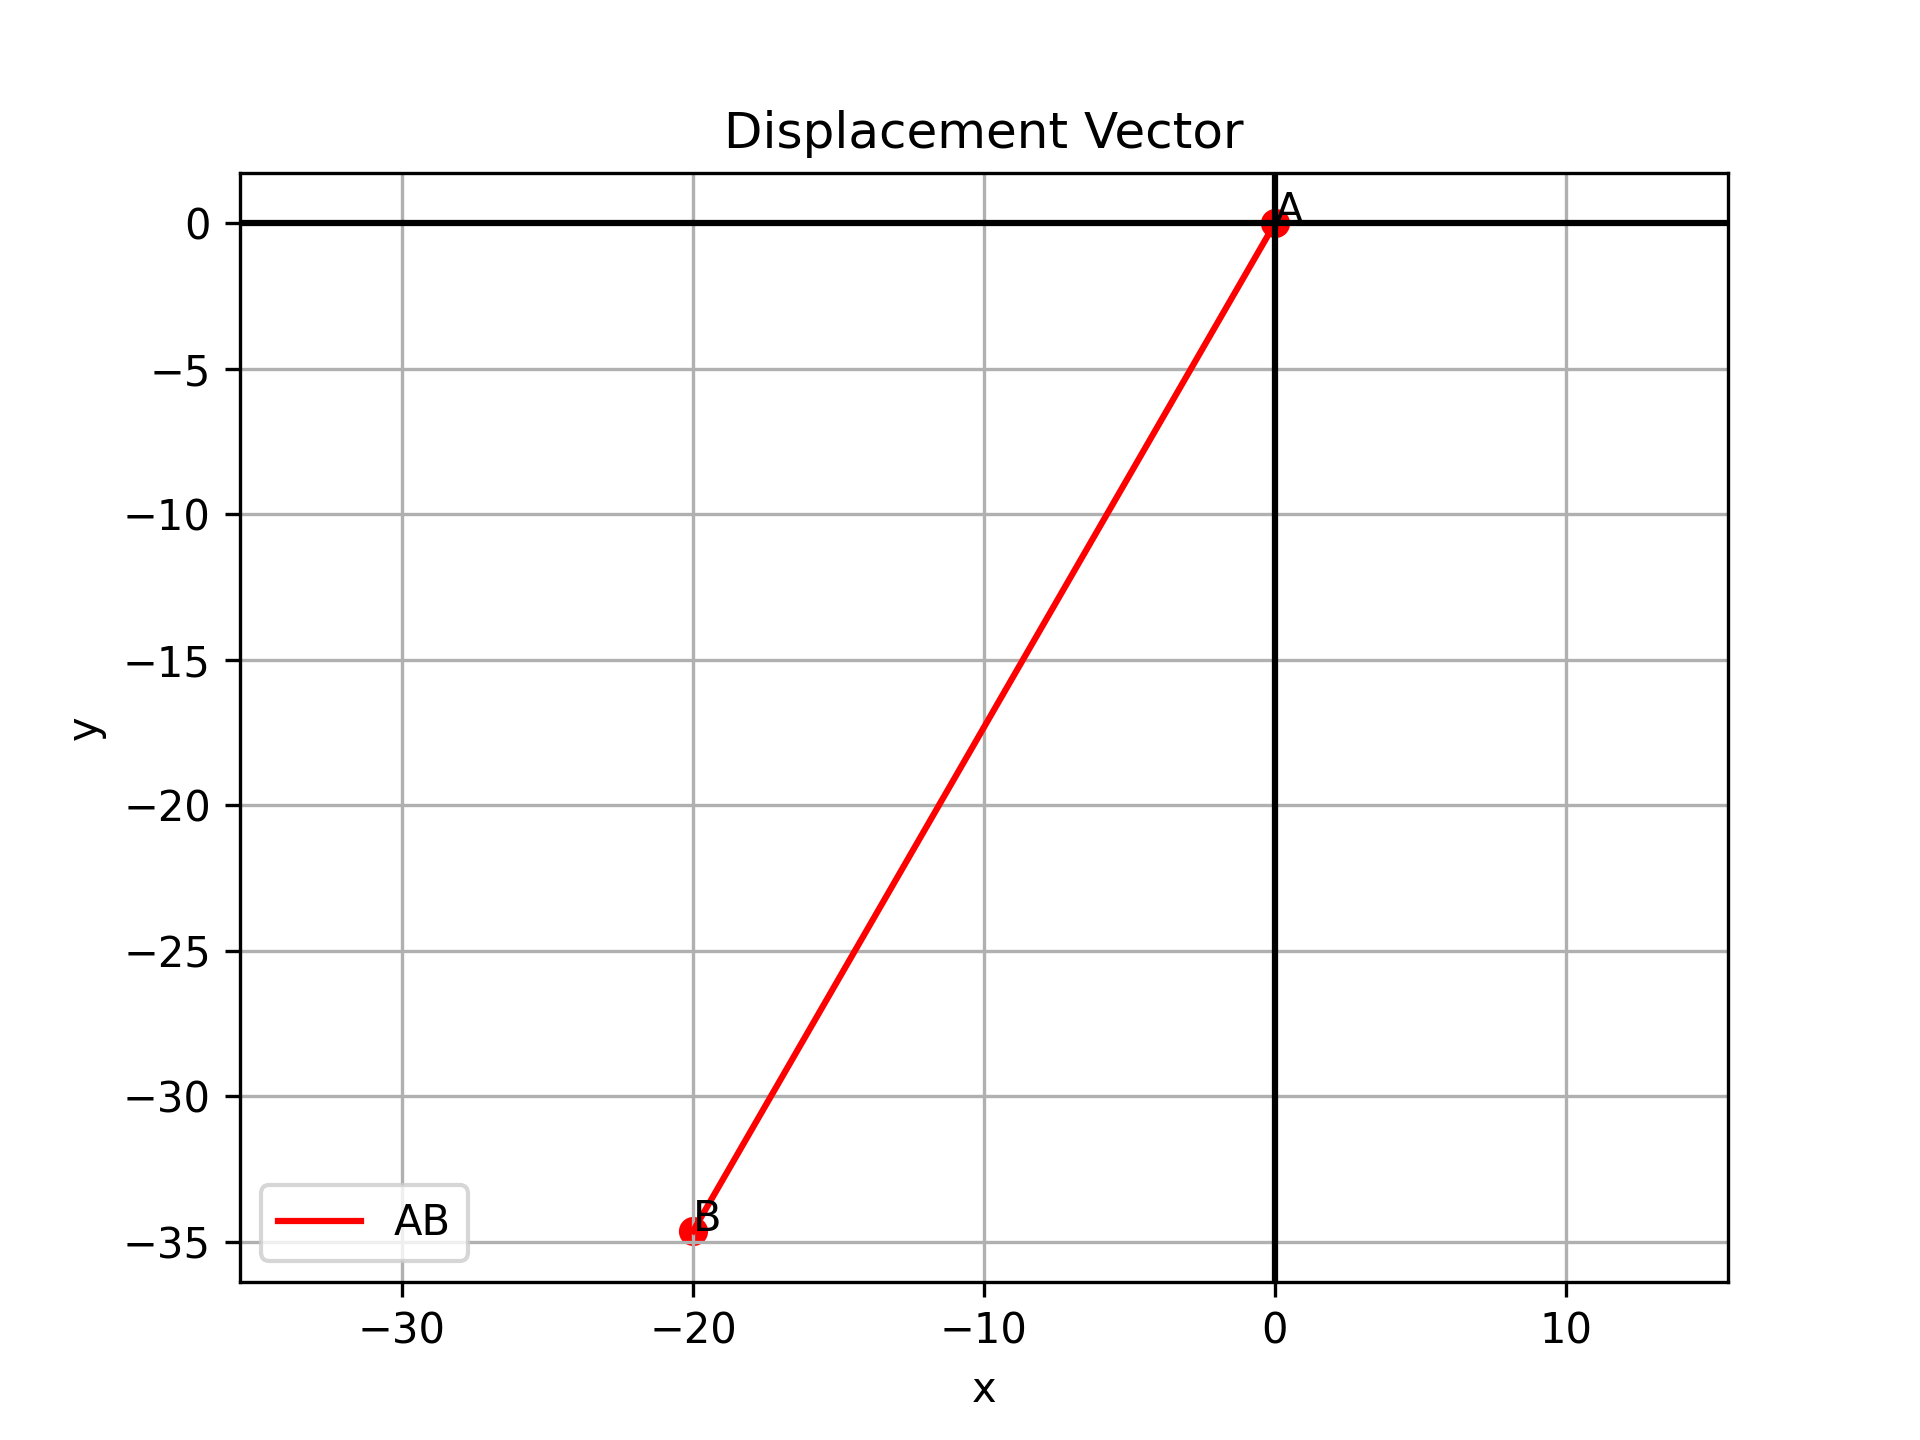
\includegraphics[width=0.6\linewidth]{figs/fig.png}
\end{center}
\end{frame}

\end{document}
